\documentclass{article} % For LaTeX2e
\usepackage{multicol}
\usepackage{nips13submit_e,times}
\usepackage{hyperref}
\usepackage{url}
\usepackage{amsmath}
\usepackage{amsfonts}
\usepackage{breakurl}
\usepackage{graphicx}
\usepackage{caption}
\usepackage{subcaption}
\usepackage{float}
\usepackage{fancyvrb}
\usepackage{booktabs}
\usepackage[font=footnotesize,labelfont=bf]{caption}
\usepackage[margin=1in]{geometry}
% \documentstyle[nips13submit_09,times,art10]{article} % For LaTeX 2.09
\bibliographystyle{ieeetr}

\title{Predicting water pump failure in Tanzania and optimising maintenance routes}


\author{
Sam Kim \\
Harvard College\\
Cambridge, MA 02138 \\
\texttt{samuelkim@college.harvard.edu} \\
\And
Gareth Haslam \\
Harvard Extension School\\
Cambridge, MA 02138 \\
\texttt{haslam.gareth@gmail.com} \\
}

% The \author macro works with any number of authors. There are two commands
% used to separate the names and addresses of multiple authors: \And and \AND.
%
% Using \And between authors leaves it to \LaTeX{} to determine where to break
% the lines. Using \AND forces a linebreak at that point. So, if \LaTeX{}
% puts 3 of 4 authors names on the first line, and the last on the second
% line, try using \AND instead of \And before the third author name.

\newcommand{\fix}{\marginpar{FIX}}
\newcommand{\new}{\marginpar{NEW}}

\nipsfinalcopy % Uncomment for camera-ready version

\begin{document}



\maketitle

\begin{abstract}
We describe MCMC techniques to model the functionality of water pumps in Tanzania and suggest an optimised route for their maintenance. Using field data describing various attributes of each pump, such as construction year, installer, and location, we describe a method to predict the current status of the pump from a set of three possibilities (functioning, functioning needs repair, and not functioning). We also optimize the route that a maintenance crew could take to repair damaged pumps in a version of the well--known, NP--hard, traveling salesman problem. We find acceptable solutions using stochastic metaheuristics. Code and more information are available at \url{http://ghaslam.github.io/AM207/}.
\end{abstract}

\begin{multicols}{2}

\section{Introduction}

Access to clean water is a fundamental need for people all over the world. Around 11\% of the world's population currently lack such access due to either lack of natural resources or lack of infrastructure \cite{UN2013}. In Tanzania, despite the availability of water, only 33.5\% have access to a piped source \cite{Morisset2012}. Many others depend on pumps for their supply. When these pumps fail, that can create serious problems for the people who depend on them. Previous work on predicting the failure of mechanical devices such as pumps has benefitted from the use of both statistical analysis as well as data obtained from direct observation of the machines, for example diagnostic vibration sensors \cite{Nakamura2007}. As the popularity of machine learning and 'big data' continues to grow, researchers are also studying how failure can be predicted based on training data from large historical datasets, for example for rod pumps in the oil industry \cite{Liu2013}. Liu's research used subject matter experts to first identify whether a pump was operating normally or about to fail and then trained their model to recognise the features in the data such as daily usage, that predicted the label. 

We aim to use Bayesian Methods to assign one of three categorical labels indicating the functional status each pump (functioning, functioning needs repair, and not functioning). The Bayesion models will be built on training data, then used to predict the functional status for wells with unknown status. Then, we treat the repair of the damaged pumps as a constrained optimisation problem over the space of all possible routes that the maintenance crew could take to reach the damaged wells. We ignore the existing road infrastructure, terrain, height etc. and assume that all locations are equally accessible. 

\section{The Data}

The data for this project was provided as part of a data science challenge run by DrivenData.org \cite{DrivenData2015}. DrivenData aims to encourage data scientists from around the world to take part in online competitions to develop predictive statistical models that can address important problems in the fields of health, international development, and the environment. The data for the Tanzanian water pump competition was aggregated from the Tanzanian Ministry of Water by Taarifa, an open source platform for tracking infrastructure related issues \cite{Taarifa2015}.  The dataset contains records of 59,400 water pumps with information on a range of 39 parameters, such as pump construction year, installer, type of pump, water quality, population around the well, cost of water, quantity and others. These include a mix of categorical and numerical data, and there are also many missing values. Each pump is assigned a unique ID as well as precise coordinates for its location. A subset of the parameters are shown in Table 1. The final column in Table 1 indicates the current status of the pump which the model will attempt to predict. The optimisation algorithm will then attempt to find the best route that reaches the damaged pumps in the second part.

\begin{table}
\caption{Sample of the DrivenData Tanzania water wells dataset}
\centering
\resizebox{\columnwidth}{!}{
\begin{tabular}{lrlrlrrrr}
\toprule
ID &         Installer        &  GPS Height & Longitude & Latitude &   Construction\_Year &  Source\_Type &  Quantity\_Type & Status\_Group  \\
\midrule
69572 &   Roman         & 1390             &       34.93 &  -9.86 &   1983 &                         Spring &          Enough  &           Functioning \\
8776 &   Grumeti          & 1399             &      34.69 &  -2.15 &   2002 &                          Rainwater &           Insufficient &          Functioning Needs Repair  \\
34310 &   World Vision & 686               &    37.46 &  -3.82 &   1967 &                           Dam &           Enough &           Functioning Needs Repair \\
67743 &   UNICEF       & 263                &   38.49 &  -11.15  &   1997 &                         Machine &           Dry &         Non-functioning \\
19728 &   Artisan          &  0                  &   31.13 &     -1.83 &   2007 &                         Rainwater &           Seasonal &           Functioning  \\
\bottomrule
\end{tabular}
}
\end{table}


In addition to the parameters given in the original dataset, we calculate some additional parameters such as age (based on the construction year), and relative remoteness (based on the average distance of the 5 nearest neighbours). Figure \ref{fig:map-phys} shows a map of the physical geography of Tanzania and another showing the locations of the pumps. The high density of pumps appears as a solid blue colour but actually represents many individual points.

\begin{figure*}
  \centering
  \begin{subfigure}[b]{0.5\textwidth}
    \centering
    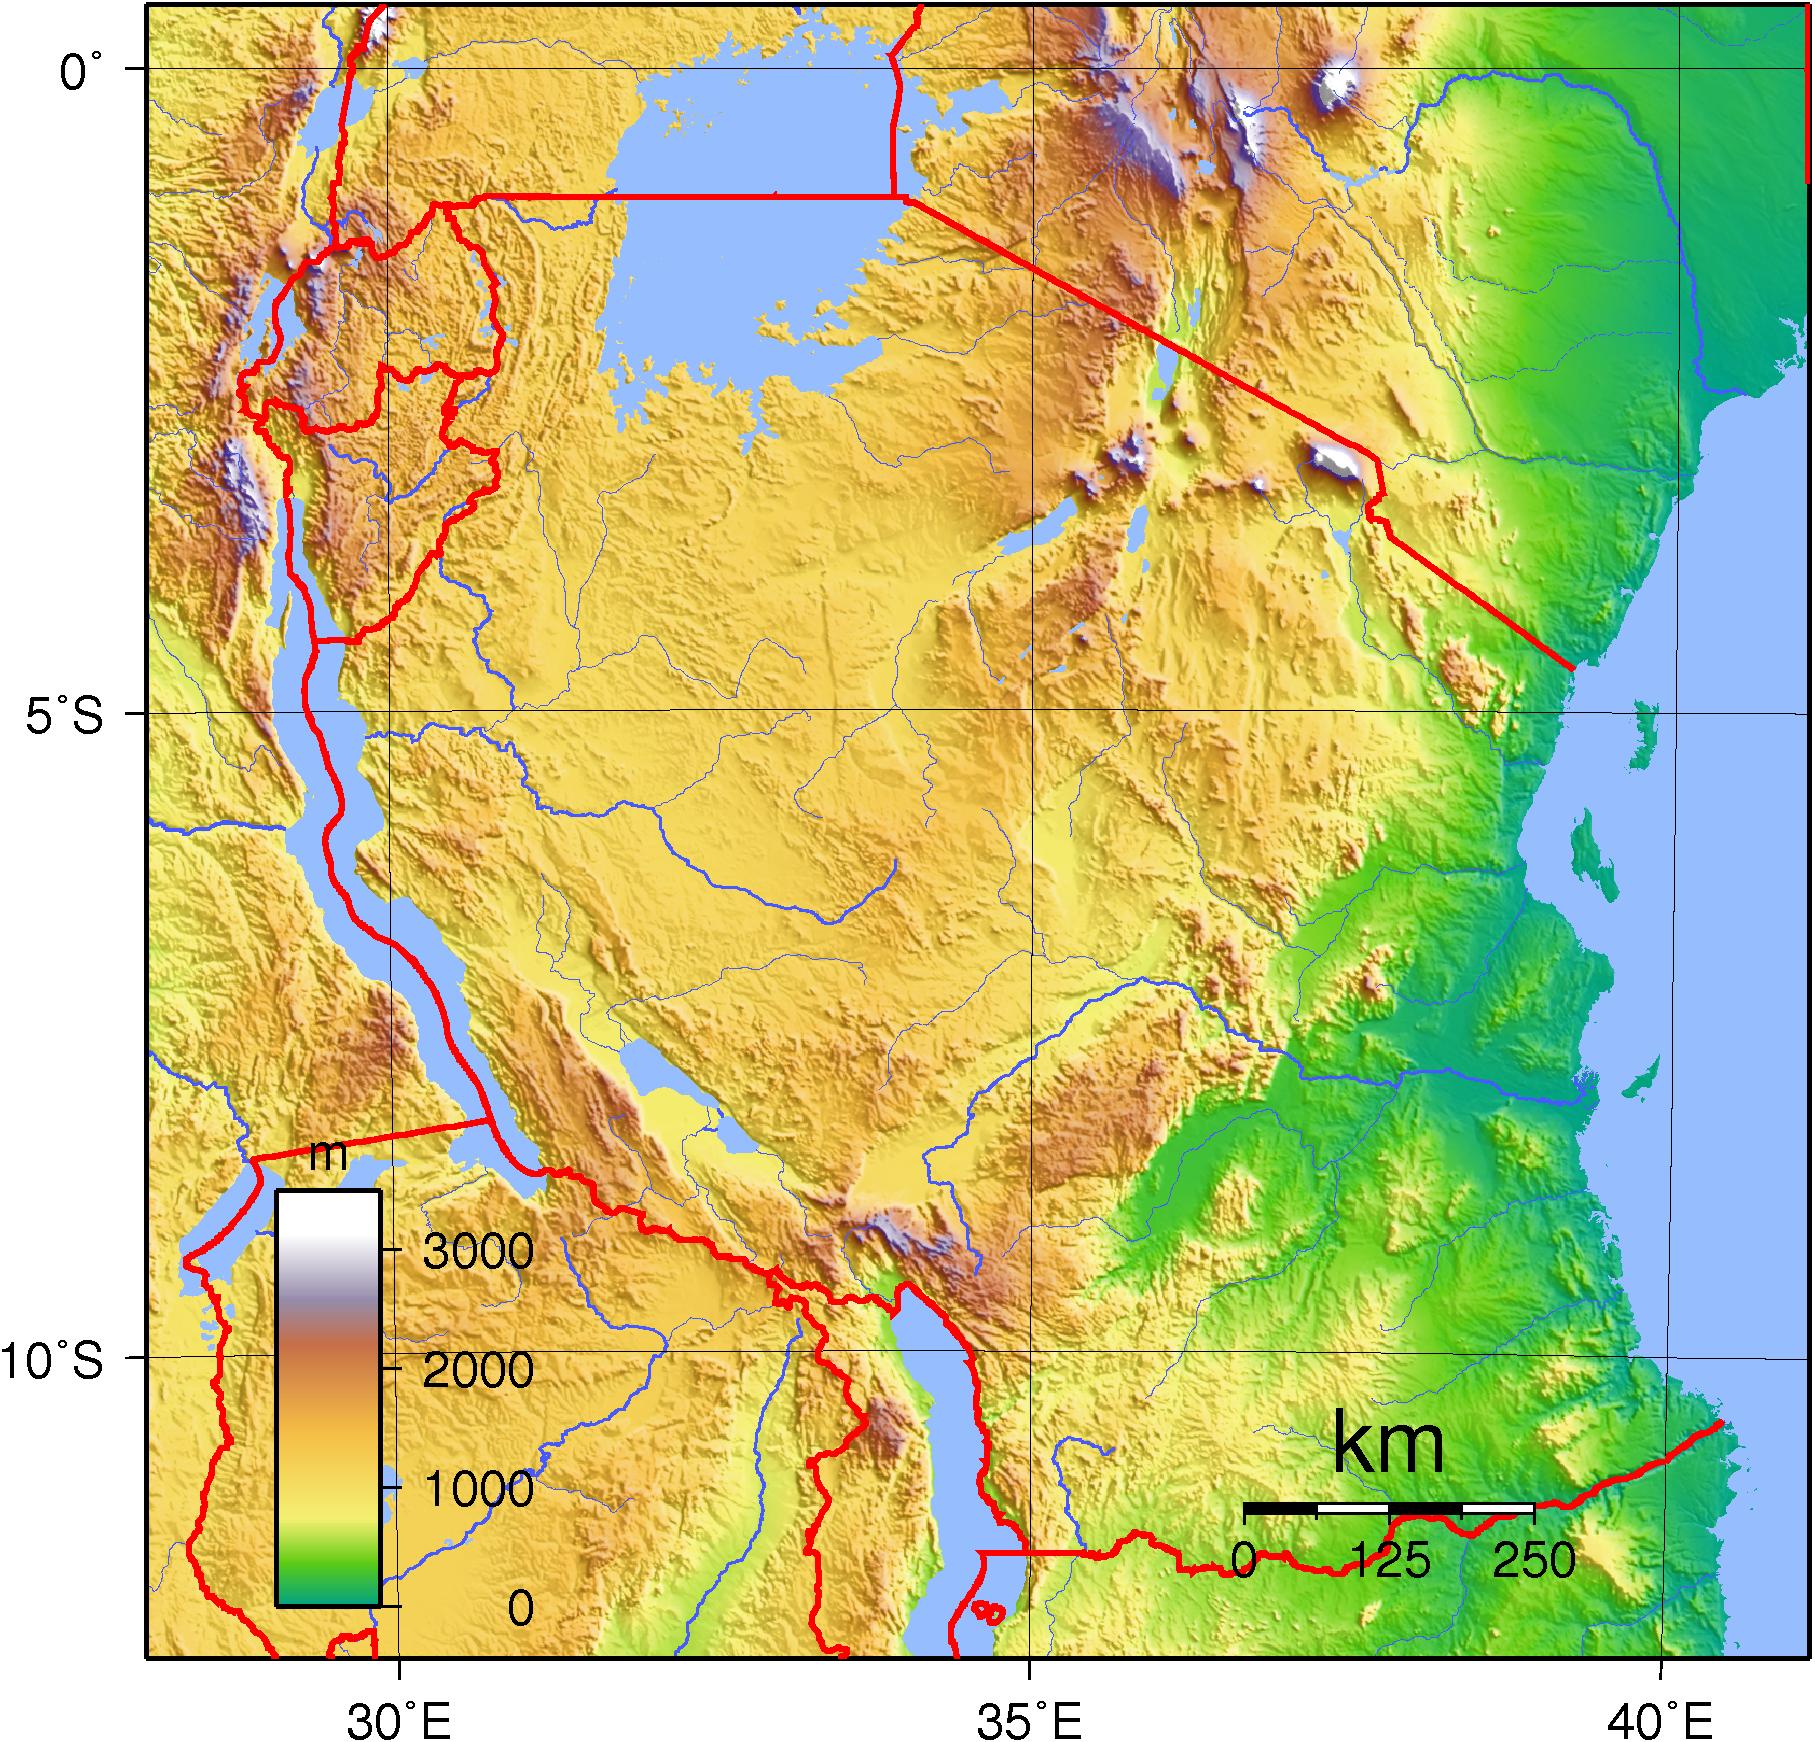
\includegraphics[width=\textwidth]{figures/Tanzania}
    \caption{Physical geography of Tanzania.}
    \label{fig:map-phys}
  \end{subfigure}~\begin{subfigure}[b]{0.5\textwidth}
    \centering
    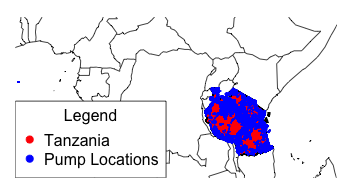
\includegraphics[width=\textwidth]{figures/PumpMap}
    \caption{Distribution of water pumps.}
    \label{fig:map-points}
  \end{subfigure}
  \caption{Geography of Tanzania and distribution of water pumps.}
  \label{fig:map}
\end{figure*}

\section{Modeling water well functionality}

\subsection{Model Classification}

Bayesian methods are only compatible with numerical data and do not work directly with classification problems, so we need to convert the categorical data and classes into numerical data and labels.

For the classification, we can take two approaches:
\begin{enumerate}
\item Assume that the 3 labels, "non functional", "functional needs repair", and "functional" lie on a spectrum where the distance between "non functional" and "functional" is greater than the difference between "non functional" and "functional needs repair" or "functional needs repair" and "functional. We can then have the Bayesian model predict a number $y$, and then convert this to a label using a range, where the exact limits can be adjusted:
\begin{align*}
\text{functional: } & 0.67\leq y_i \\
\text{functional needs repair: } & 0.33<y_i<0.67 \\
\text{non functional: } &  y_i \leq 0.33
\end{align*}
\item The assumption that the 3 labels lie on a linear spectrum is not necessarily a safe assumption, and the limits are set rather arbitrarily. A more natural and common method in machine learning is to build a classifier that decides between 2 classes. In this case, we can either build 3 one-versus-one classifiers or 3 one-versus-rest classifiers and use majority vote (or probabilities in the case of a tie) to make the final classification.
\end{enumerate}

We use the first approach for its simplicity, although further work would investigate the performance of the second approach, which is much more versatile at the cost of computational complexity.

During the training stage of our model, we also need to convert the given labels into numbers. Assuming that we use the first approach above for prediction, we use a similar scheme:
\begin{equation*}
y_i = 
\begin{cases}
0 & \text{ non functional}\\
0.5 & \text{ functional needs repair}\\
1 & \text{ functional}
\end{cases}
\end{equation*}

\subsection{Categorical data}

Many of the data features are categorical data that do not have any numerical interpretation, so we cannot convert them the same way that we converted our label. For example, the "installer" feature has labels such as "UNICEF," "Roman," and "Artisan." To deal with these, we use one-of-k representation in which we add a new feature column for every unique value. For example, we would add the columns "installer=UNICEF," "installer=Roman," and "installer=Artisan." The "installer=UNICEF" would be 1 if that data's "installer" was "UNICEF," and 0 otherwise. So if there are $k$ unique values for a particular categorical feature, then for each data point, we add on a vector of length $k$ which has a single 1 and $k-1$ 0s.

\subsection{The model}

We model $y_i$ using a logistic function that constrains the range to $0 < y_i < 1$, and the parameter for the logistic function is controlled by the features and weights, which are also parameters that we need to calculate. Our model comes from the assumption that there are certain factors impacting decay rate, and so the functionality is dependent on this decay rate.
We then select features from the data which we have a prior belief to have a strong influence on functionality, choose priors on their distributions and construct a Metropolis-Hastings Sampler to select the optimum value for each parameter. New predictions of functionality can then be made from this model.

We also add on a term for noise, $\epsilon_i$, which we assume is Gaussian noise controlled by the standard deviation $\sigma$.

\begin{gather*}
y_i = \frac{1}{1+e^{\alpha_i}}+\sigma\epsilon_i \\
\alpha_i = \beta_0 + \beta_1 x_{i,1} + \beta_2 x_{i,2} + ... + \beta_n x_{i,n}
\end{gather*}

There are $n$ features and $n+2$ parameters ($n+1$ $\beta$s and $\sigma$). The parameters are found by sampling from the posterior:

\begin{equation*}
p(Y,\Theta)=p(Y|\Theta)p(\Theta)
\end{equation*}

\section{Prediction Results}

\subsection{Results}

\begin{figure*}
	\begin{subfigure}{0.5\textwidth}
		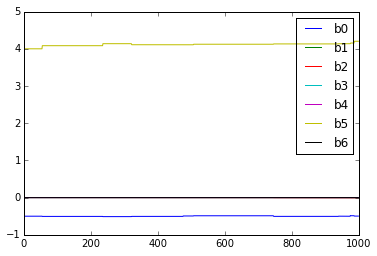
\includegraphics[width=\textwidth]{figures/trace_block}
		\caption{Blockwise updating}
		\label{fig:trace_block}
	\end{subfigure}
	\begin{subfigure}{0.5\textwidth}
		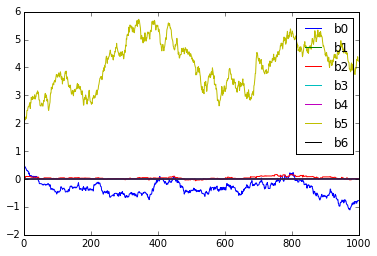
\includegraphics[width=\textwidth]{figures/trace_component}
		\caption{Componentwise updating}
		\label{fig:trace_comp}
	\end{subfigure}
	\caption{Traceplot of model parameters, using MH sampler.}
	\label{fig:trace}
\end{figure*}

Figure~\ref{fig:trace} shows the trace plot of the model parameters with blockwise updating and componentwise updating. These are after the burn-in period. Blockwise updating has an acceptance rate of nearly 0 because we are updating 8 parameters at a time. Componentwise updating has a much higher acceptance rate, although at a huge time cost.

The parameters chosen are "longitude," "latitude," "age" (2015-"construction\_year"), "gps\_height," "quantity=dry," and "population."

We see that $\beta_5$ has significant predictive power since this is the farthest from 0. This corresponds to the "quantity=dry" feature. $\beta_0$ is the constant offset, which we would expect to be non-zero. 

By fine-tuning the step parameters and carefully choosing features, we reach a cross-validation prediction accuracy of 60.6\%.

\subsection{Comparison to machine learning approaches}

Here we compare our methods with other common machine learning methods.

The k-Nearest Neighbors algorithm (also known as the k-NN algorithm) is a machine learning algorithm that can be applied to classification problems. There is no training aspect to the algorithm. Predictions are made by taking the $k$ nearest data points to the desired data point in feature space, and taking the majority of their labels. The labels can also be weighted by $1/d$, where $d$ is the distance from the desired data point to the labeled data point. We apply the k-NN algorithm using only the longitude and latitude data, so we are picking the geographically nearest neighbors. Accuracy in cross-validation is shown in the below figure as a function of $k$. We see that it reaches 69\% prediction accuracy.

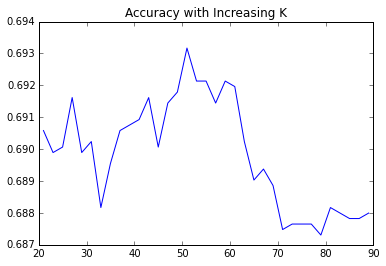
\includegraphics[width=8cm]{figures/kNN_accuracy_vs_K.png}

Decision trees are a machine learning method in which a tree of rules is built. One traverses down the tree, and each node represents a rule based on the data's features. The leaves are the final decision. The nodes are built based on which features have the most predictive power for classification. Random forests are an extension of decision trees in which many trees are trained, and stochasticity is introduced to make the trees different, which decreases bias. We show in randomforest\_explore.ipynb that random forests on a small subset of features can reach an accuracy of 79\%. Further experimentation and more sophisticated feature extraction can reach prediction accuracies of 83\% on this data.

Bayesian modeling is probably not the best method to use for this type of problem. It assumes that the classification can be described by some sort of model, and we would have to guess this model ahead of time. Decision trees and random forests do not assume any sort of relation between the variable features and the labels, and merely seek out the variable features with the highest predictive power. Second, there are a lot of parameters in the MH sampler that need to be tuned, including initial guesses for the parameters and step sizes. Additionally, Bayesian modeling takes extremely long to train, on the order of hours on a laptop, assuming that the initial guesses for the parameters and step sizes are set correctly. Training k-NN and random forests take on the order of minutes.

\section{Optimizing maintenance crew route}

In the second part of this project, we aim to suggest an optimised route by which a maintenance crew could visit the damaged pumps. The choice of locations can either be taken from the originally labeled pumps or based on the outputs of our model's labels. 

\subsection{The traveling salesman problem}

Having hopefully identified a method for accurately predicting which pumps will fail, we can imagine that the Tanzanian Ministry of Water will want to task a maintenance crew with visiting each of these locations. We may also assume that the maintenance crew are based in the commercial capital of Dar Es Salaam. The crew wishes to visit all $N$ locations in as efficient manner as possible. This problem is equivalent to the traveling salesman problem (TSP), first described in 1932 by Karl Menger \cite{Menger}. A compact mathematical formulation of the problem is given by Miller et. al. \cite{Miller1960} as follows:


\begin{align*}
\textrm{Find variables }& X_{ij}  \textrm{ and } U_i i,j = 1, 2, \cdots , n \textrm{ that minimize}:\\
Z &= \min \sum_{i=0}^n \sum_{j\ne i,j=0}^n C_{ij} X_{ij}\\
\end{align*}

\begin{align*}
\textrm{subject to} & \\
	& \sum_{i=1}^n X_{ij} = 1 && j = 1, 2 , \cdots, n \\
	& \sum_{j=1}^n X_{ij} = 1 && i = 1, 2, \cdots, n \\
	&U_i - U_j + nX_{ij} \le n-1 && i, j = 2, \cdots, n i\ne j \\
	& x_{ij} \in \{0, 1\} && i,j=0, \cdots, n \\
\end{align*}

The optimal solution is subject to the following constraints:

\begin{itemize}
  \item $X_{ij}$ is a binary decision variable indicating whether to accept a move from location $i$ to location $j$.
  \item $C_{ij}$ is the distance between location $i$ and location $j$.
  \item The objective function is the sum of the distances for routes that we decide to take.
  \item Each location is visited once and only once.
\end{itemize}

The difficulty with solving the TSP is that for large numbers of locations, it becomes impossible to test all possible routes as the problem has $\mathcal{O}$$(n!)$ complexity and is classified as NP-hard. Therefore, it can be sufficient to find an answer that is 'good enough' even if it is not globally optimal. To find  this 'good enough' solution we use Simulated Annealing (SA). 

Figure \ref{fig:TSP} shows the effect of simulated annealing on reducing the total distance travelled by the maintenance crew and suggest a near-optimal route between the pumps in need of repair. Due to the large number of locations, only a subset are shown in order to make viewing easier. The depot in Dar Es Salaam is highlighted in red. The trace plot shown in \ref{fig:Plain-TSP-Trace} shows that the SA algorithm has approached a stable route distance which is significantly shorter than the original random route.

\begin{figure*}
	\begin{subfigure}{0.5\textwidth}
		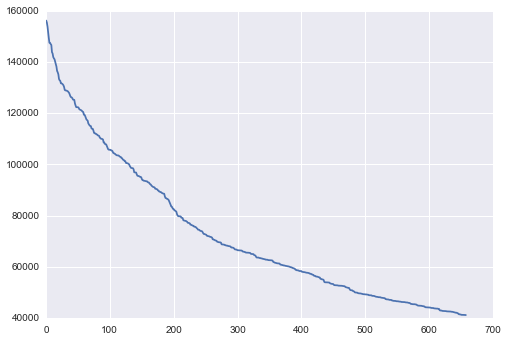
\includegraphics[width=\textwidth]{figures/Plain-TSP-Trace}
		\caption{Decrease in distance due to annealing}
		\label{fig:Plain-TSP-Trace}
	\end{subfigure}
	\begin{subfigure}{0.5\textwidth}
		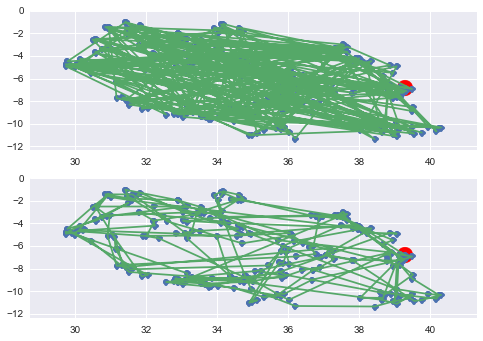
\includegraphics[width=\textwidth]{figures/Optimised-Route}
		\caption{Optimised maintenance route with Dar Es Saleem in red.}
		\label{fig:trace_comp}
	\end{subfigure}
	\caption{Simulated annealing for travelling salesman.}
	\label{fig:TSP}
\end{figure*}

\subsection{Modifications}

With one maintenance crew, the total distance travelled is 41,000 km, which is obviously too much for one crew to travel. It is also important to note that we use the Haversine formula for calculating the distance between locations as the straight-line, Euclidean distance is imprecise for large distances on a sphere \cite{Sinnot1983}. An obvious extension of the problem is to imagine that instead of making a single visiting every pump, the crew make multiple trips, returning to the depot in Dar Es Salaam each time (or equivalently, that multiple crews leave and return to the depot each day). This leads to a decrease in total distance travelled from 41,000 km to 34,500 km. This problem is commonly referred to as the vehicle routing problem (VRP). Gavish et. al. describe a range of other interesting formulations of the TSP which would be relevant to our situation \cite{Gavish1978}. Finally, we looked at prioritising the damaged pumps that were identified as being 'remote', with the assumption that people depending on these pumps would have fewer alternative sources nearby that they could visit if their own pump failed. We first identified the average distance from each pump to its 5 nearest neighbours using the k-dimensional tree method. We then added this weight to the cost function used by the SA algorithm. As expected, this led to a significant reorganisation of the route and an increase in the total distance travelled but with the benefit of reaching those in need more quickly. The effect of these modifications are show in \ref{fig:Modifications}.

\begin{figure*}
	\begin{subfigure}{0.5\textwidth}
		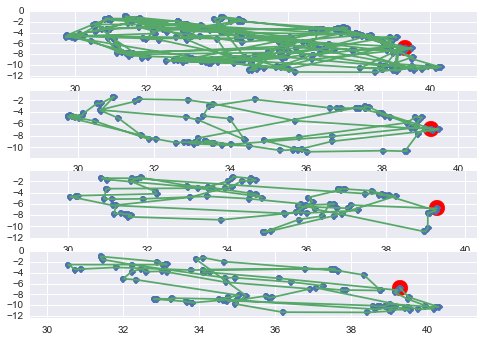
\includegraphics[width=\textwidth]{figures/Multiple-salesmen}
		\caption{Effect of adding multiple maintenance crews.}
		\label{fig:Multiple-crews}
	\end{subfigure}
	\begin{subfigure}{0.5\textwidth}
		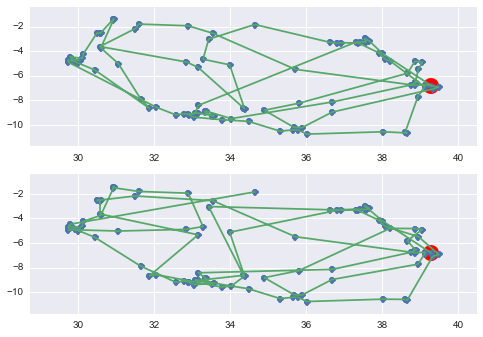
\includegraphics[width=\textwidth]{figures/Prioritising-remote-pumps}
		\caption{Optimised maintenance route for prioritising more remotes pumps.}
		\label{fig:Priority-remote}
	\end{subfigure}
	\caption{Adding multiple maintenance crews and prioritising remote pumps.}
	\label{fig:Modifications}
\end{figure*}

It would be interesting in future work on this data to look at solving the Knapsack Problem to simulate the maintenance crew having a constrained amount of materials to allocate to each pump repair and also the selection of the optimal position of the depot. Another interesting exercise would be to look at how alternative solutions for the TSP compare in terms of both processing time and distance -- for example Genetic Algorithms have been used successfully to solve the TSP.

\section*{Conclusions}

We have shown that Bayesian modelling can produce predictions for the operating status of water pumps that are significantly better than the naive baseline prediction. The approach assumes an a priori model of how the pump functions based on parameters that we believe to be significant and then updates the relative strength of each of these parameters probabilistically to converge towards to optimal values. However, we have also shown that other Machine Learning Methods can produce superior predictions based on simpler assumptions. Having developed methods for identifying faulty pumps we have demonstrated the use of simulated annealing to optimise the route that a maintenance crew can take and added constraints such as a fixed depot, and multiple crews. Interesting avenues for future work have also been suggested. 

\bibliography{Write-up_Ref}

\end{multicols}
\end{document}